\chapter{Introduction}
\lecture{1}{04/10/2021}


\section{Qubits}
The \textbf{bit} is the fundamental concept of classical computation and information. Quantum computation and information are built upon an analogous concept: the \textbf{quantum bit}, or \textbf{qubit}. What is a qubit? Quantum mechanically, a qubit is any two-level system. For example, we can use the two different polarizations of a photon, the alignment of a nuclear spin in a
uniform magnetic field, or the two states of an electron orbiting a single atom or molecule (ammonia-based quantum computer\footnote{Ferguson, A., Cain, P., Williams, D., \& Briggs, G. (2002). Ammonia-based quantum computer. Phys. Rev. A, 65, 034303.}). Just as a classical bit has a \textbf{state} - either 0 or 1 - a qubit also has a \textbf{state}. Two possible states for a qubit are the state $|0\rangle$ and $|1\rangle$ (we use \textit{Dirac notation}\footnote{Also known as bra-ket notation, it is a formalism introduced by Paul Dirac to describe one quantum state. The name derives from the fact that the scalar product of two states $\phi$ and $\psi$ is denoted with a bracket $\langle\phi|\psi\rangle$ consisting of two parts: $\langle\phi|$ the \textit{bra} and $|\psi\rangle$ the \textit{ket}.}). The difference between bits and qubits is that a qubit can be in a state other than $|0\rangle$  or $|1\rangle$. It is also possible to form \textit{linear combinations} of states, often called \textit{superpositions}:

\begin{equation*}
    |\psi\rangle=\alpha|0\rangle + \beta|1\rangle
\end{equation*}

The numbers $\alpha$ and $\beta$ are complex numbers. See in another way, the state of a qubit is a vector in a two-dimensional complex vector space. The special states $|0\rangle$ and $|1\rangle$ are know as computational basis states and form an orthonormal basis for this vector space. We can examine a bit to determine whether it is in the state 0 or 1. For example, computers do this all-time when they retrieve the contents of their memory. Instead, quantum mechanics tells us that we can only acquire much more restricted information about the quantum state. When we measure a qubit, we get either 0 with probability $\alpha$ or 1 with probability $\beta$. Naturally, they must satisfy the following condition:

\begin{equation*}
    |\alpha|^2+|\beta|^2=1
\end{equation*}

Like in a QM system, the phase is irrelevant, it's a degree of freedom. For this reason, qubits could store infinite information. However, this conclusion turn out to be misleading, because of the behavior of a qubit when observed. Remind that the measurement of a qubit will give only either 0 or 1. Furthermore, measurement changes the state of a qubit, collapsing it from its superposition of $|0\rangle$ and $|1\rangle$ to the specific state consistent with the measurement result. From a single measurement one obtains only a single bit of information about the state of the qubit, thus resolving the apparent paradox. It turns out that only if infinitely many identically prepared qubits were measured would one be able to determine $\alpha$ and $\beta$ for a qubit in the state $|\psi\rangle$.

\subsection*{Summary for general principles on QM}
\begin{itemize}
    \item \textbf{Postulate I}: What is a state? We use Dirac notation to represents a vector in an Hilbert-space (finite dimension) $|\psi\rangle \in \mathcal{H}$, where the states lives. The states is given by a vector also named as \textit{ray} and it should have a unit norm (conservation of probability) $|| |\psi\rangle ||=1$. All phases are irrelevant $|\psi\rangle \approx e^{i\alpha}|\psi\rangle \ \alpha\in\mathbb{R}$, if two states differs from a phase, they have the same physical effect.
\end{itemize}
If we have two states $|\psi_1\rangle$ and $|\psi_2\rangle$, and we consider their linear combination: $|\psi\rangle = \alpha_1|\psi_1\rangle+\alpha_2|\psi_2\rangle$, then $|\psi\rangle$ is also a state in $\mathcal{H}$. But we need to pay attention for $|\psi\rangle$, we need to normalize it for the conservation of probability.

\begin{definition}{Scalar product}
    We define \textbf{scalar product} the following quantity: $\langle\phi|\psi\rangle$ (\textbf{bra-ket} notation), where $\langle\phi|$ is the dual vector of $|\phi\rangle$.
\end{definition}

\noindent Qubit systems work in $\mathcal{H}=\mathbb{C}^2$. Where a vector $\begin{pmatrix}z_1\\z_2\end{pmatrix}$ has $z_1,z_2\in\mathbb{C}$. We can also say that $|0\rangle$ and $|1\rangle$ are an orthogonal bases:

\begin{equation*}
    |0\rangle = \begin{pmatrix}1\\0\end{pmatrix} \ \ \ \ \ |1\rangle = \begin{pmatrix}0\\1\end{pmatrix}
\end{equation*}

\noindent where their scalar products are:

\begin{equation*}
    \langle0|0\rangle=\langle1|1\rangle=1 \ \ \ \ \ \langle0|1\rangle=\langle1|0\rangle=0
\end{equation*}

\noindent So our general state it can be written as:

\begin{equation*}
    \begin{pmatrix}z_1\\z_2\end{pmatrix}=z_1\begin{pmatrix}1\\0\end{pmatrix} + z_2\begin{pmatrix}0\\1\end{pmatrix}=z_1|0\rangle+z_2|1\rangle
\end{equation*}

\noindent The scalar product between $|\phi\rangle=\begin{pmatrix}z_1\\z_2\end{pmatrix}$ and $|\psi\rangle=\begin{pmatrix}w_1\\w_2\end{pmatrix}$ is defined as:

\begin{equation*}
    \langle\psi|\phi\rangle=w_1^*z_1+w_2^*z_2
\end{equation*}

\noindent If we have $|\phi\rangle = \begin{pmatrix}z_1\\z_2\end{pmatrix}$ (ket), we transpose and conjugate $\langle\phi|=(z_1^*, z_2^*)$ (bra). Then we can rewrite the scalar product as:

\begin{equation*}
    \langle\psi|\phi\rangle=(w_1^*, w_2^*)\begin{pmatrix}z_1\\z_2\end{pmatrix}=w_1^*z_1+w_2^*z_2
\end{equation*}

\noindent Summing up, we can write a generic state as:
\begin{equation*}
    \begin{pmatrix}z_1\\z_2\end{pmatrix}=z_1|0\rangle+z_2|1\rangle
\end{equation*}

\noindent with these two constraints:
\begin{itemize}
    \item \textbf{Conservation of probability}: $|z_1|^2+|z_2|^2=1$
    \item \textbf{Phase invariance}: $\begin{pmatrix}z_1\\z_2\end{pmatrix}=e^{i\alpha}\begin{pmatrix}z_1\\z_2\end{pmatrix} \Rightarrow \begin{matrix}z_1\approx e^{i\alpha}z_1 \\z_2 \approx e^{i\alpha}z_2\end{matrix}$
\end{itemize}
\noindent Obtaining
\begin{equation*}
    |\psi\rangle =z_1|0\rangle+z_2|1\rangle
\end{equation*}
\noindent Using the \textbf{conservation of probability}:
\begin{equation*}
    |\psi\rangle =\cos\frac{\theta}{2}e^{i\phi_1}|0\rangle+\sin\frac{\theta}{2}e^{i\phi_2}|1\rangle
\end{equation*}
\noindent Using the \textbf{phase invariance}, so long as $\phi_1$ and $\phi_2$ still arbitrary, we have a freedom by multplying for a phase $e^{i\alpha}$\footnote{The global phase is physically irrelevant, while the relative phase is physically important for certain phenomena like interference.}:
\begin{equation*}
    |\psi\rangle =\bigg(\cos\frac{\theta}{2}e^{i\phi_1}|0\rangle+\sin\frac{\theta}{2}e^{i\phi_2}|1\rangle\bigg)e^{i\alpha}
\end{equation*}
\noindent Redefining $\phi_1=-\alpha$ and $\phi = \phi_2+\alpha$ we get the general parametrization of a general qubit:
\begin{equation*}
    |\psi\rangle= \cos\frac{\theta}{2}|0\rangle+\sin\frac{\theta}{2}e^{i\phi}|1\rangle
\end{equation*}

\subsection{Bloch sphere}
We can visualize the generic state of a qubit using the spherical coordinates and with the introduction of a unit vector $\vec n = (\sin \theta \cos \phi, \sin \theta \sin \phi, \cos \theta)$, we get the \textbf{Bloch sphere} (note also as $S^2$ unit sphere).

\begin{figure}[!ht]
    \centering
    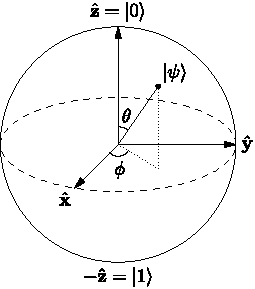
\includegraphics{images/chapter1/Bloch_Sphere.pdf}
    \caption{General rappresentation of a qubit state $|\psi\rangle$ on the Bloch sphere}
    \label{fig:BlochSphere}
\end{figure}

\noindent Each state coincides with each point present on the surface of the sphere, there is a one-to-one correspondence between a point on the surface and a state $|\psi\rangle$. We must underline the fact that the scalar product which we define in $\mathbb{C}^2$ is different from the scalar product in $S^2$, because, in the last one, $|0\rangle$ and $|1\rangle$ are in the same direction but opposite verse, so their scalar product is equal to -1 while in $\mathbb{C}^2$ is equal to 0. The Bloch sphere is a useful technique to visualize the qubit states.
\newpage
\lecture{2}{08/10/2021}